\begin{center}
\underline{\Large{T.P.N°3: Flexión Simple}}
\end{center}

\begin{enumerate}
\item a) Dimensionar una viga de 5 m de longitud perteneciente a un sistema de vigas de un pórtico de hormigón armado que se encontrará sometida a un momento flector en el tramo generado por cargas permanentes de MD = 3,5 tnm y por sobrecargas de ML = 2 tnm. En el apoyo, MD = 4 tnm y ML = 3 tnm. El hormigón será H-25 y el acero ADN 42/50. La viga se encuentra expuesta a un ambiente clase CL. Efectuar el cálculo según Reglamento CIRSOC 201-05 y CIRSOC 201-82.
b) Dibujar la sección de la viga.
\item Dimensionar analíticamente a flexión la viga V102 de la Figura 1 construida de hormigón armado de sección T y 5 m de largo, ubicada entre dos losas en una dirección de 15 cm de espesor cuyas luces son de 2,5 m y 2 m entre ejes de vigas cada una. La carga total por peso propio de la losa es de 850 kg/m2, mientras que la sobrecarga es de 200 kg/m2. Para el cálculo considerar el peso propio de la viga y las reacciones transmitidas por las losas.
Efectuar el cálculo según CIRSOC 201-82 o bien según CIRSOC 201-05.
\begin{figure}[H]
\begin{center}
     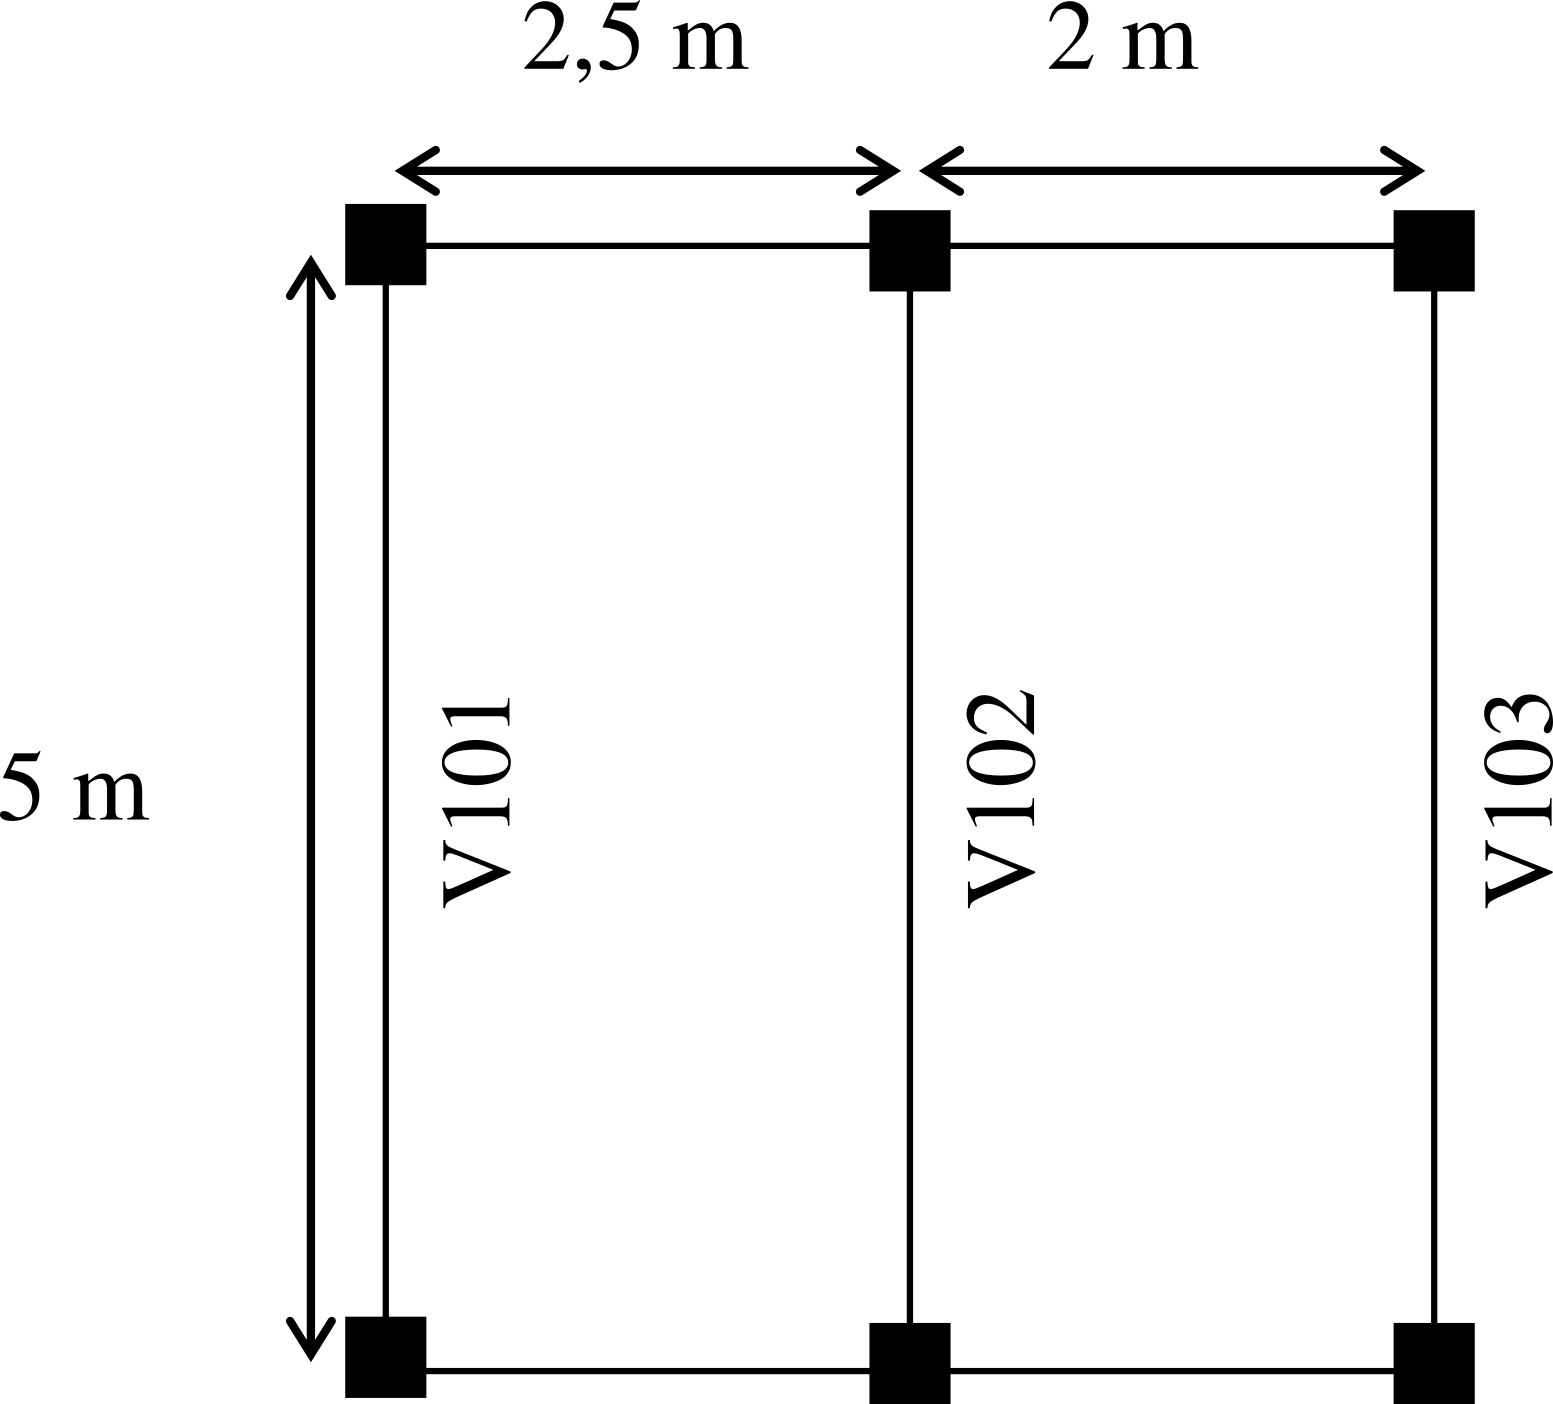
\includegraphics[scale = 0.9]{chapters/chapter_1/images/figura1.png}
\caption{Esquema de cálculo para la viga V102}
\end{center}
\end{figure}

\item Indicar el momento último que es capaz de resistir la viga de la Figura 2, cuya armadura principal es de 4$\phi$16 mm construida con hormigón H-20 y acero ADN 42/50. Despreciar el aporte de las barras superiores. Realizar el cálculo según el CIRSOC 201-05.
\begin{figure}[H]
\begin{center}
     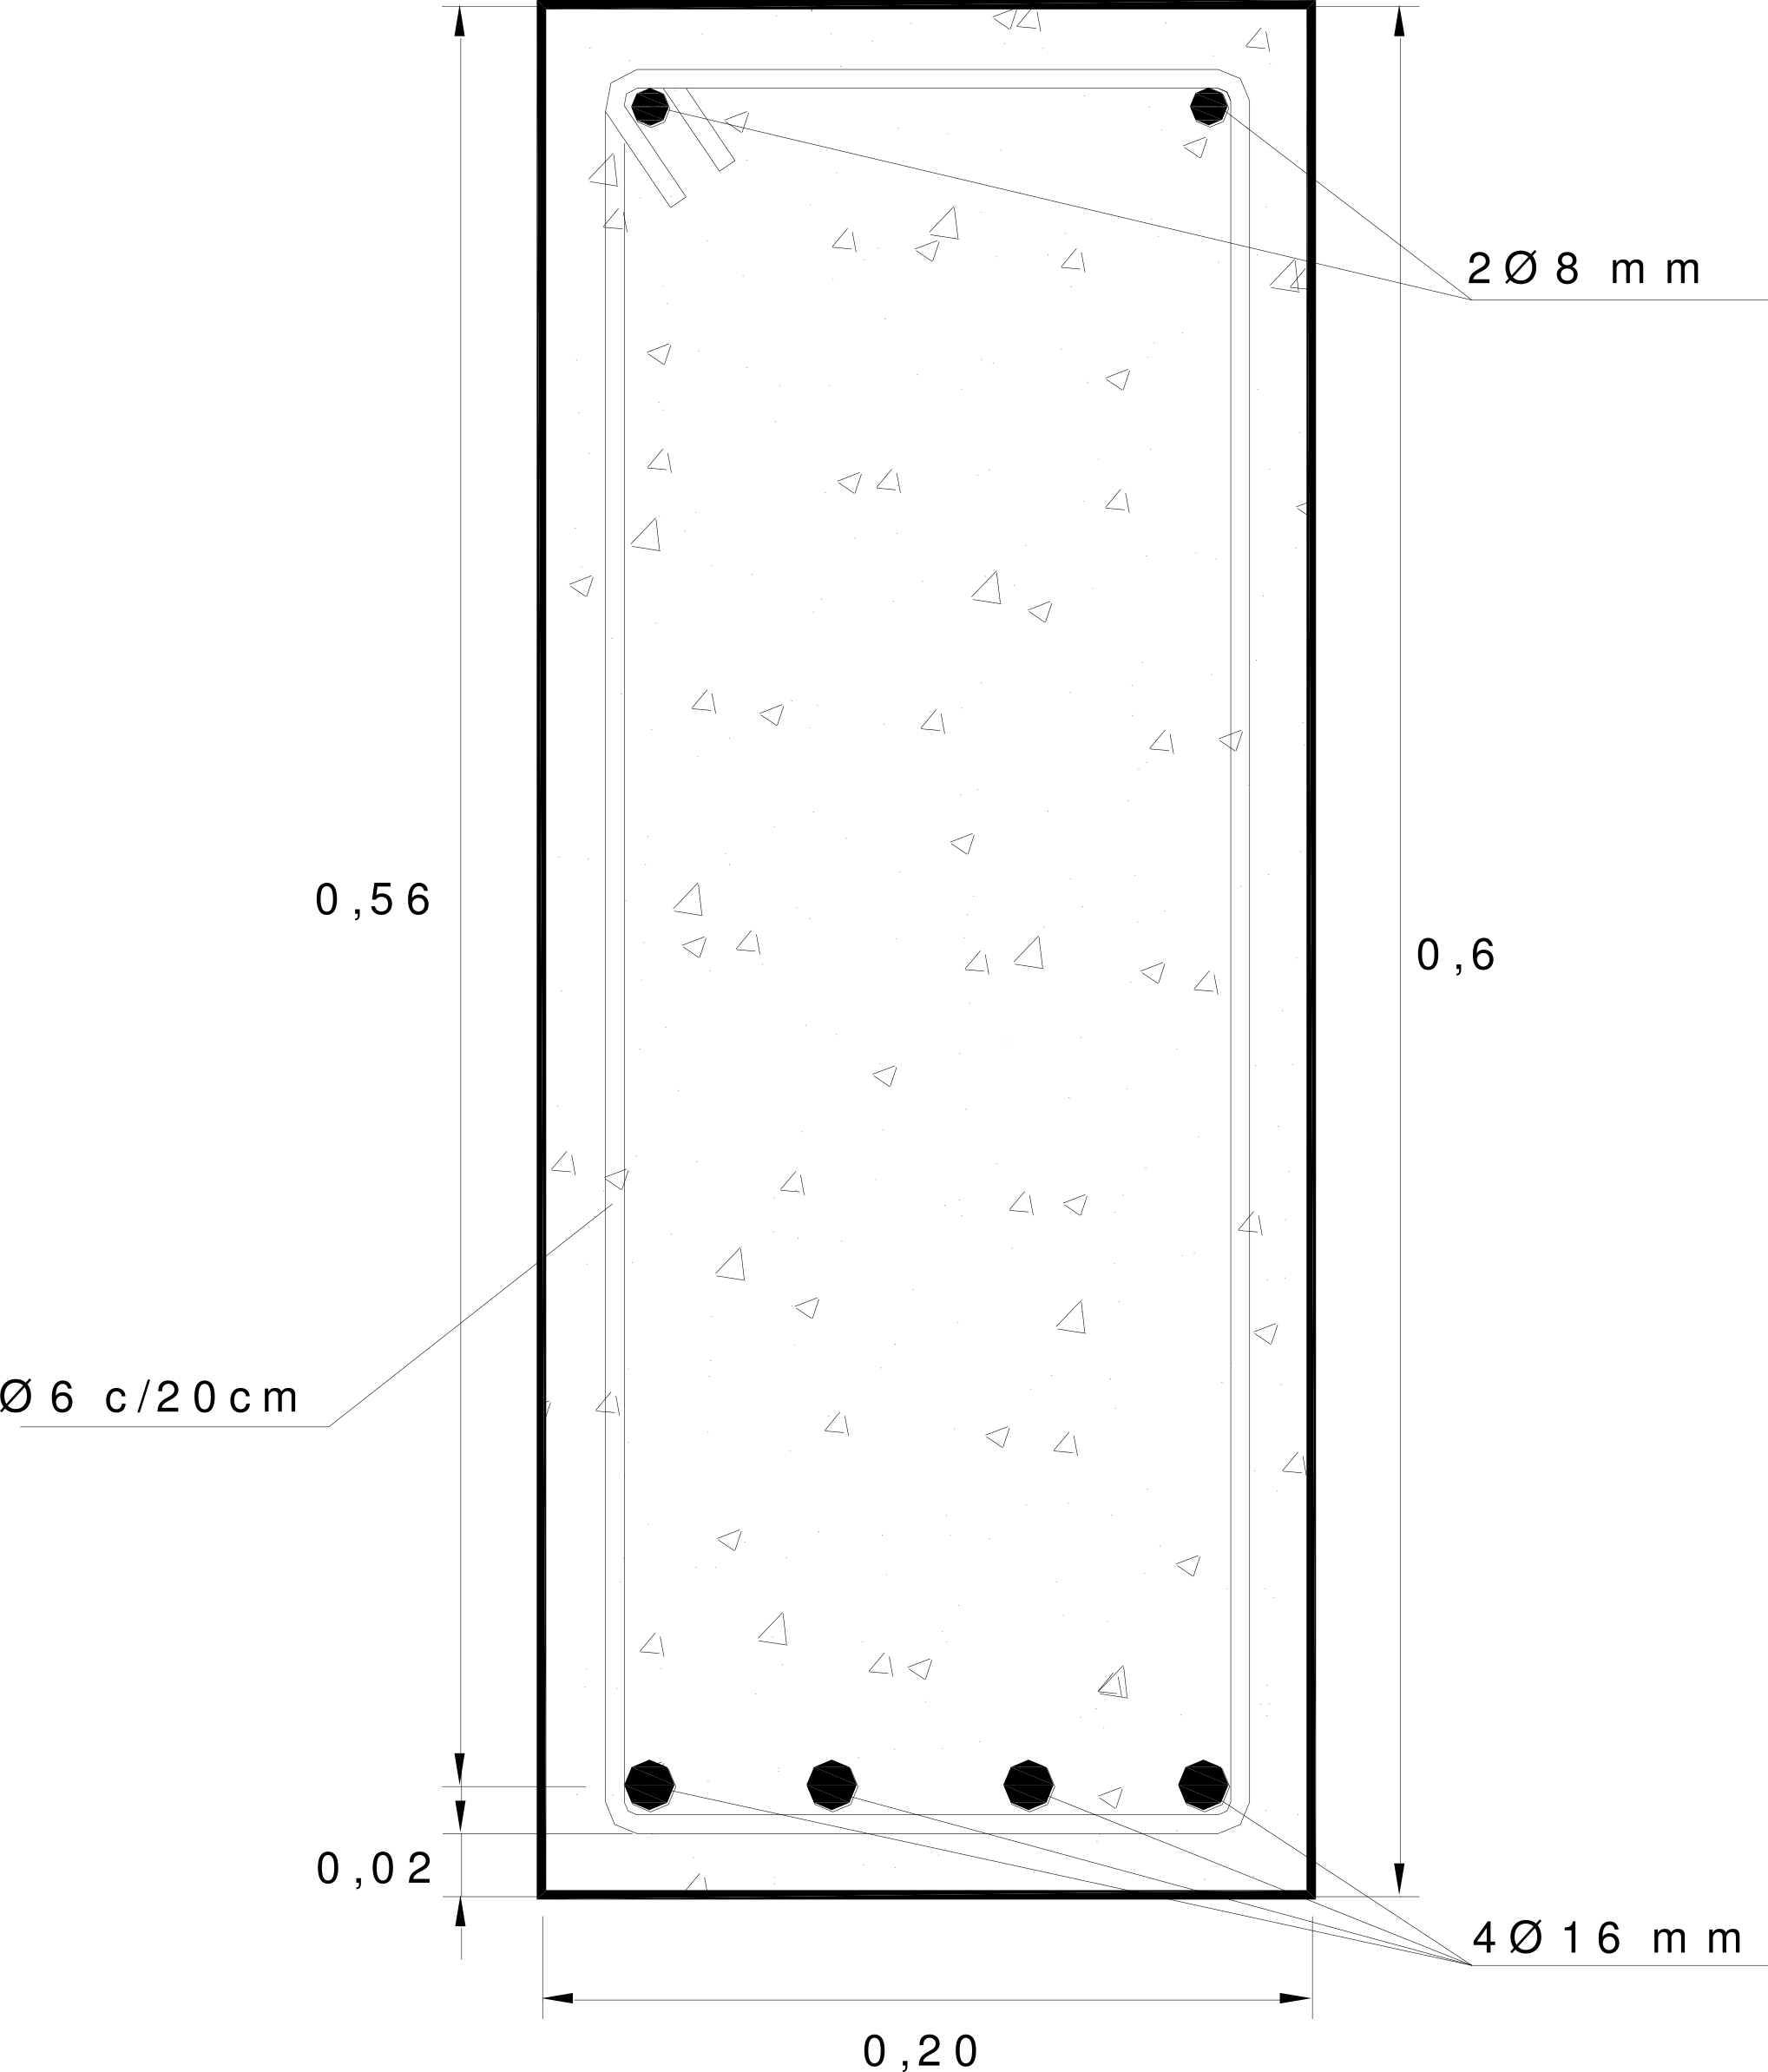
\includegraphics[scale = 0.9]{chapters/chapter_1/images/figura2.png}
     \caption{Corte de la viga del ejercicio 3)}
\end{center}
\end{figure}
\end{enumerate}


\begin{enumerate}
\item \underline{Dimensionar una viga de 5m de longitud}

\underline{Datos:}\\
\begin{align*}
& l=5m\\
& \text{\underline{Para el tramo:}}\\
& M_D=3.5 t.m\\
& M_L=2 t.m\\
& \text{\underline{Para el apoyo:}}\\
& M_D=4 t.m\\
& M_L=3 t.m
\end{align*}

Hormigón H-25 $\Rightarrow f'c = 250 \frac{Kg}{cm^2} = 25 MPa$\\
Acero ADN 42/50 $\Rightarrow fy = 4200 \frac{Kg}{cm^2} = 420 MPa$\\
Exposición CL (cloruros), de tabla tenemos el recubrimiento en vigas más un $50\% \Rightarrow Cc=3cm$\\

\newpage
\begin{itemize}
\item \underline{Armadura Inferior en el tramo}

\begin{align*}
& M_u = 1.2 \cdot M_D + 1.6 \cdot M_L = 1.2 \cdot 3.5 t.m + 1.6 \cdot 2 t.m = \framebox{$7.4 t.m$}\\
& M_n = \frac{M_u}{\phi} = \frac{7.4 t.m}{0.9} = 8.22 t.m \Rightarrow \framebox{$822000 Kg.cm$}
\end{align*}
Para hallar la altura útil se estiman los siguientes valores:\\
\[\left\{ \begin{array}{ll}
         h \approx \frac{l}{10} = \frac{5m}{10} = 50 cm & \\
         b_w \approx \frac{h}{2} = \frac{50 cm }{2} = 25 cm \quad \text{adopto} \Rightarrow b_w = 20 cm &\\
         dbe = 6 mm &\\
         db = 16 mm & \end{array} \right. \]
\begin{align*}
& d = h - Cc - dbe - \frac{db}{2} = 50cm - 3cm -0.6cm -\frac{1.6cm}{2} = \framebox{$45.6cm$}\\
& m_n = \frac{M_n}{0.85 \cdot f'c \cdot b_w \cdot d^2} = \frac{822000 Kg.cm}{0.85 \cdot 250 \frac{Kg}{cm^2} \cdot 20 cm \cdot (45.6cm)^2} = \framebox{0.093}\\
& Ka = 1- \sqrt{1-2 \cdot m_n} = 1- \sqrt{1-2 \cdot 0.093} = \framebox{0.0978}\\
& Ka_{min}= \frac{1.4}{0.85 \cdot f'c} = \frac{1.4}{0.85 \cdot 25MPa} = \framebox{0.0658}\\
& Ka_{max}= 0.375 \cdot \beta_1 = 0.375 \cdot 0.85 = \framebox{0.3187}\\
& Ka_{min} < Ka < Ka_{max}\\
& 0.0658 < 0.0978 < 0.3187 \Rightarrow \quad \text{Verifica} \quad \surd\\
& As= 0.85 \cdot f'c \cdot b_w \cdot Ka \cdot \frac{d}{fy} = 0.85 \cdot 250 \frac{Kg}{cm^2} \cdot 20cm \cdot 0.0978 \cdot \frac{45.6cm}{4200 \frac{Kg}{cm^2}} = \framebox{$4.51 cm^2$}\\
& \text{Adopto} \quad 4 \phi 12mm \Rightarrow 4.52cm^2 \quad \text{inferiores}\\
& \text{Separacion} = \frac{b_w-2 \cdot Cc - 2 \cdot dbe - 4 \cdot db}{3} \\ 
& = \frac{20cm-2 \cdot 3cm - 2 \cdot 0.6cm - 4 \cdot 1.2cm}{3} = \framebox{$2.66cm > 2.5 cm$} \quad \Rightarrow \text{Verifica} \quad \surd
\end{align*}

\begin{figure}[H]
\begin{center}
     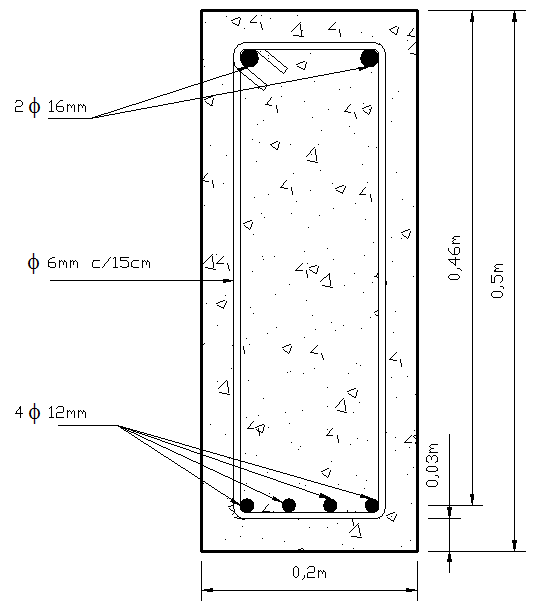
\includegraphics[scale = 0.5]{chapters/chapter_1/images/figura3.png}
     \caption{Sección en el tramo}
\end{center}
\end{figure}

\item \underline{Armadura Superior en el apoyo}
\begin{align*}
& M_u = 1.2 \cdot M_D + 1.6 \cdot M_L = 1.2 \cdot 4 t.m + 1.6 \cdot 3 t.m = \framebox{$9.6 t.m$}\\
& M_n = \frac{M_u}{\phi} = \frac{9.6 t.m}{0.9} = 10.66 t.m \Rightarrow \framebox{$1066000 Kg.cm$}\\
& m_n = \frac{M_n}{0.85 \cdot f'c \cdot b_w \cdot d^2} = \frac{1066000 Kg.cm}{0.85 \cdot 250 \frac{Kg}{cm^2} \cdot 20 cm \cdot (45.6cm)^2} = \framebox{0.1207}\\
& Ka = 1- \sqrt{1-2 \cdot m_n} = 1- \sqrt{1-2 \cdot 0.1207} = \framebox{0.1290}\\
& Ka_{min}= \frac{1.4}{0.85 \cdot f'c} = \frac{1.4}{0.85 \cdot 25MPa} = \framebox{0.0658}\\
& Ka_{max}= 0.375 \cdot \beta_1 = 0.375 \cdot 0.85 = \framebox{0.3187}\\
& Ka_{min} < Ka < Ka_{max}\\
& 0.0658 < 0.1290 < 0.3187 \Rightarrow \quad \text{Verifica} \quad \surd\\
& As= 0.85 \cdot f'c \cdot b_w \cdot Ka \cdot \frac{d}{fy} = 0.85 \cdot 250 \frac{Kg}{cm^2} \cdot 20cm \cdot 0.1290 \cdot \frac{45.6cm}{4200 \frac{Kg}{cm^2}} = \framebox{$5.95 cm^2$}\\
& \text{Adopto} \quad 3 \phi 16mm \Rightarrow 6.03cm^2 \quad \text{superiores}\\
& \text{Separacion} = \frac{b_w-2 \cdot Cc - 2 \cdot dbe - 3 \cdot db}{2} \\ 
& = \frac{20cm-2 \cdot 3cm - 2 \cdot 0.6cm - 3 \cdot 1.6cm}{2} = \framebox{$4cm > 2.5 cm$} \quad \Rightarrow \text{Verifica} \quad \surd
\end{align*}

\begin{figure}[H]
\begin{center}
     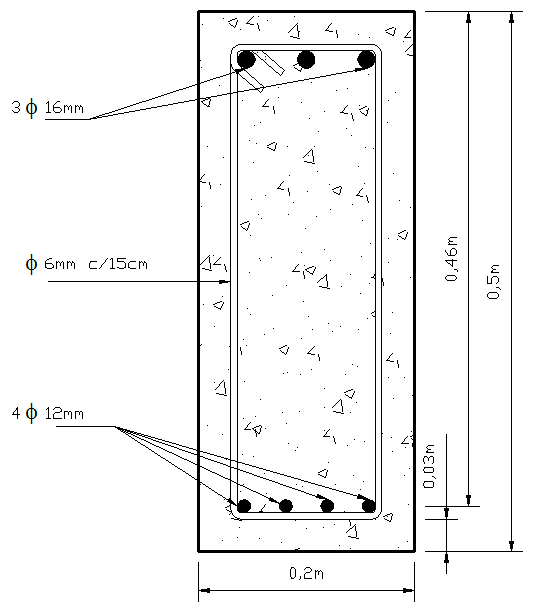
\includegraphics[scale = 0.5]{chapters/chapter_1/images/figura4.png}
     \caption{Sección en el apoyo}
\end{center}
\end{figure}

\end{itemize}


\item \underline{Viga T - Viga 102}

\underline{Datos:}\\
\begin{align*}
& l=5m\\
& h_f=15cm\\
& L_{T1}=2.5m\\
& L_{T2}=2m\\
& D_{losa}=850 \frac{Kg}{m^2}\\
& L_{losa}=200 \frac{Kg}{m^2}
\end{align*}

\begin{figure}[H]
\begin{center}
     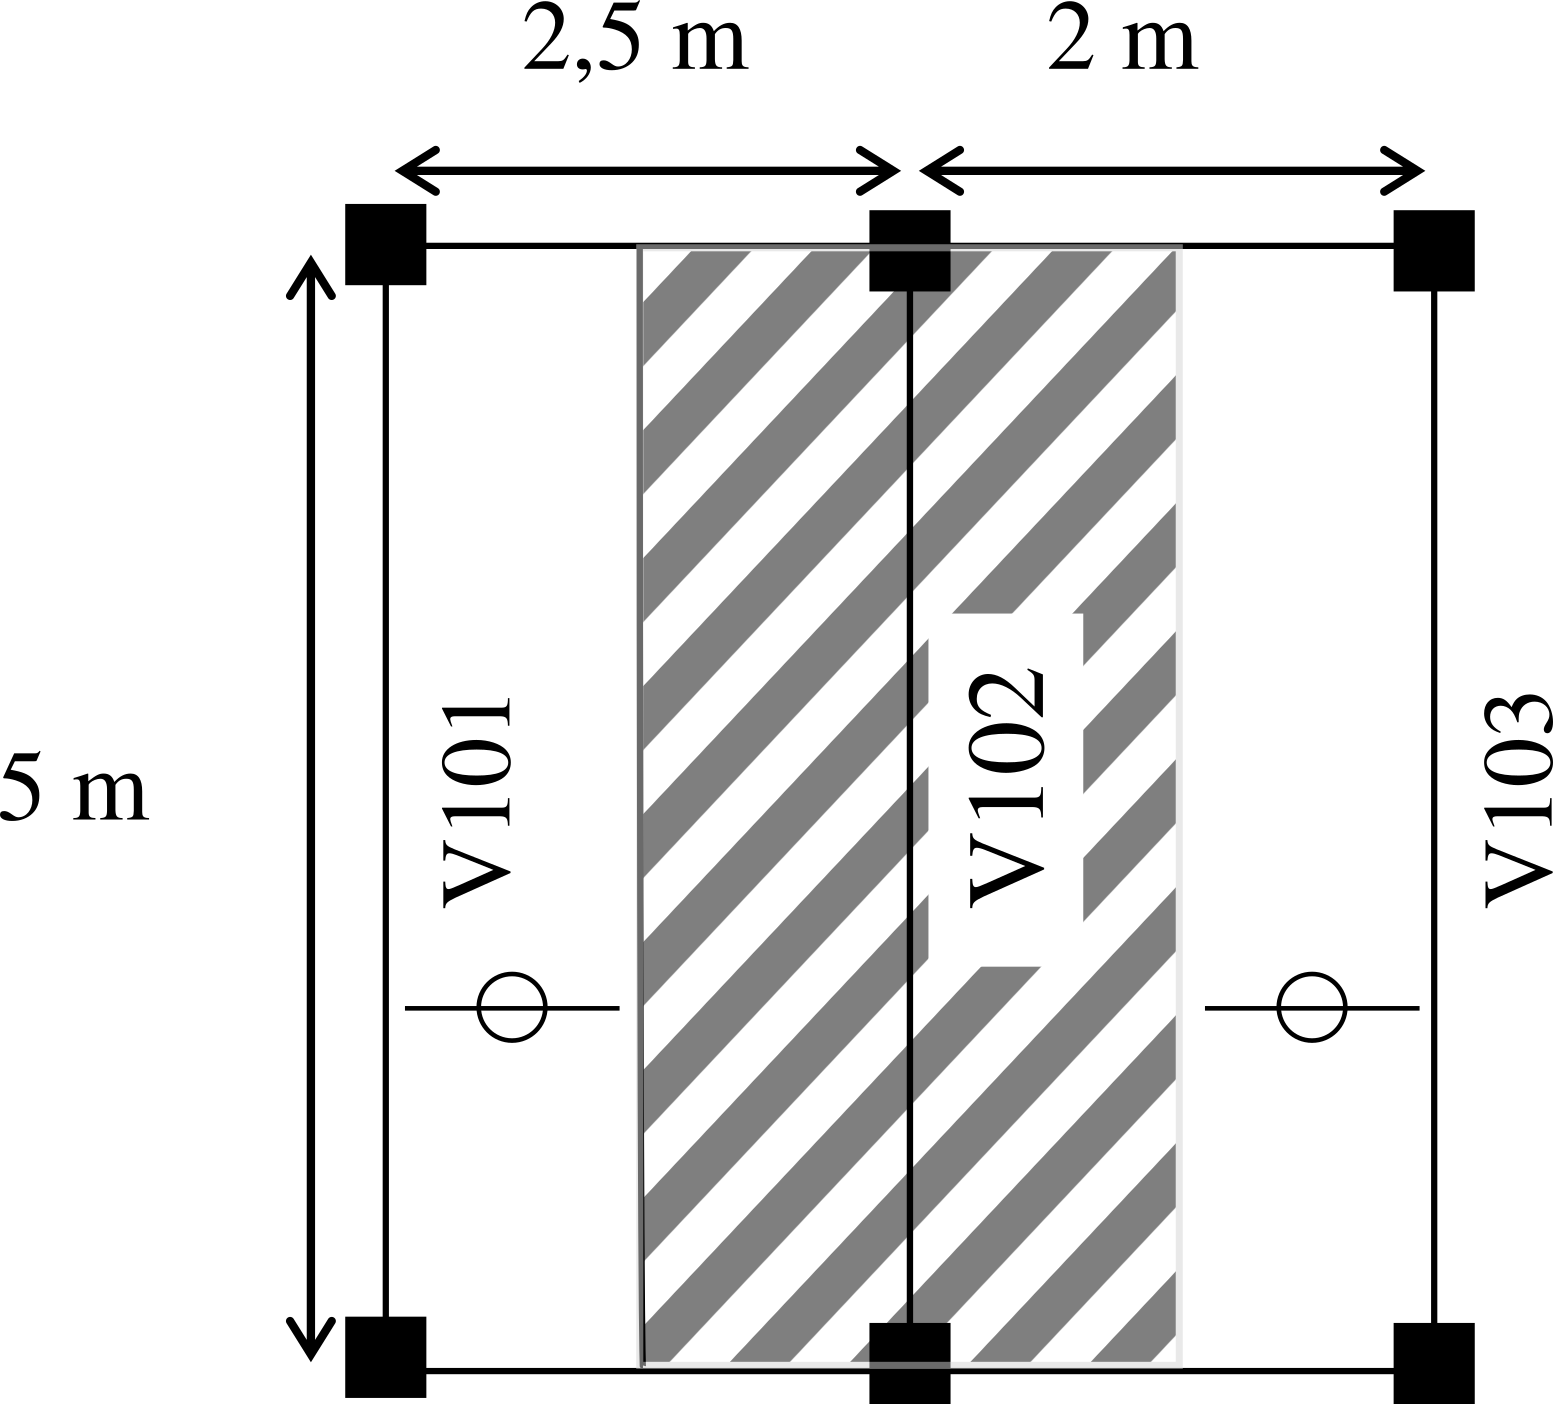
\includegraphics[scale = 0.9]{chapters/chapter_1/images/figura5.png}
     \caption{Vista en planta}
\end{center}
\end{figure}

\begin{align*}
& R_D=850 \frac{Kg}{m^2} \cdot \frac{2.5m}{2}+850 \frac{Kg}{m^2} \cdot \frac{2m}{2}=\framebox{$1912.6 \frac{Kg}{m}$}\\
& R_L=200 \frac{Kg}{m^2} \cdot \frac{2.5m}{2}+200 \frac{Kg}{m^2} \cdot \frac{2m}{2}=\framebox{$450 \frac{Kg}{m}$}
\end{align*}

Para hallar la altura útil se estiman los siguientes valores:\\
\[\left\{ \begin{array}{ll}
         h \approx \frac{l}{10} = \frac{5m}{10} = 50 cm & \\
         b_w \approx \frac{h}{2} = \frac{50 cm }{2} = 25 cm \quad \text{adopto} \Rightarrow b_w = 20 cm &\\
         dbe = 6 mm &\\
         db = 12 mm & \\
         Cc = 2cm & \end{array} \right. \]
\begin{align*}
& d = h - Cc - dbe - \frac{db}{2} = 50cm - 2cm -0.6cm -\frac{1.2cm}{2} = \framebox{$46.8cm$}\\
& \text{Peso propio de la viga}\\
& D_{viga}= b_w \cdot h \cdot \gamma_{H°} = 0.2m \cdot 0.50m \cdot 2500 \frac{Kg}{m^3} = \framebox{$250 \frac{Kg}{m}$}\\
& U = 1.2 \cdot (R_D+D_{viga}) + 1.6 \cdot R_L = 1.2 \cdot (1912.6 \frac{Kg}{m}+250 \frac{Kg}{m}) + 1.6 \cdot 450 \frac{Kg}{m} = \framebox{$3315 \frac{Kg}{m}$}\\
& M_u \simeq \frac{U \cdot l^2}{8} = \frac{3315 \frac{Kg}{m} \cdot (5m)^2}{8} = \framebox{$10360 Kg.m$}\\
& M_n = \frac{M_u}{\phi} = \frac{10360 Kg.m}{0.9} = \framebox{$11511 Kg.m$}\\
& b = b_w + b_{ef_{izq}} + b_{ef_{der}}
\end{align*}

\[b_{ef_{izq}} \leq \left\{ \begin{array}{ll}
         8 \cdot h_f = 8 \cdot 0.15m = \framebox{1.2m} & \\
         \frac{l_{transversal}}{2}=\frac{2.5m}{2}=1.25m & \end{array} \right. \]

\[b_{ef_{der}} \leq \left\{ \begin{array}{ll}
         8 \cdot h_f = 8 \cdot 0.15m = 1.2m & \\
         \frac{l_{transversal}}{2}=\frac{2m}{2}=\framebox{1m} & \end{array} \right. \]

\begin{align*}
& b = b_w + b_{ef_{izq}} + b_{ef_{der}} \leq \frac{l}{4}\\
& b = 0.2m+1.2m+1m \leq \frac{5m}{4}\\
& 2.4m \leq 1.25m \quad \text{No Verifica}\\
& m_n = \frac{M_n}{0.85 \cdot f'c \cdot b \cdot d^2} = \frac{1151100 Kg.cm}{0.85 \cdot 250 \frac{Kg}{cm^2} \cdot 125 cm \cdot (46.8cm)^2} = \framebox{0.0197}\\
& Ka = 1- \sqrt{1-2 \cdot m_n} = 1- \sqrt{1-2 \cdot 0.0197} = \framebox{0.020}\\
& As= 0.85 \cdot f'c \cdot b \cdot Ka \cdot \frac{d}{fy} = 0.85 \cdot 250 \frac{Kg}{cm^2} \cdot 125cm \cdot 0.020 \cdot \frac{46.8cm}{4200 \frac{Kg}{cm^2}} = \framebox{$5.91 cm^2$}\\
& \text{Adopto} \quad 3 \phi 16mm \Rightarrow \framebox{$6.03cm^2$} \quad \text{inferiores}\\
& As_{min}=1.4 \cdot b_w \cdot \frac{d}{fy}= 1.4 \cdot 0.20m \cdot \frac{0.468m}{420MPa}= 3.12cm^2\\
& As = 6.03cm^2 > 3.12cm^2 \quad \text{Verifica} \quad \surd
\end{align*}

\begin{figure}[H]
\begin{center}
     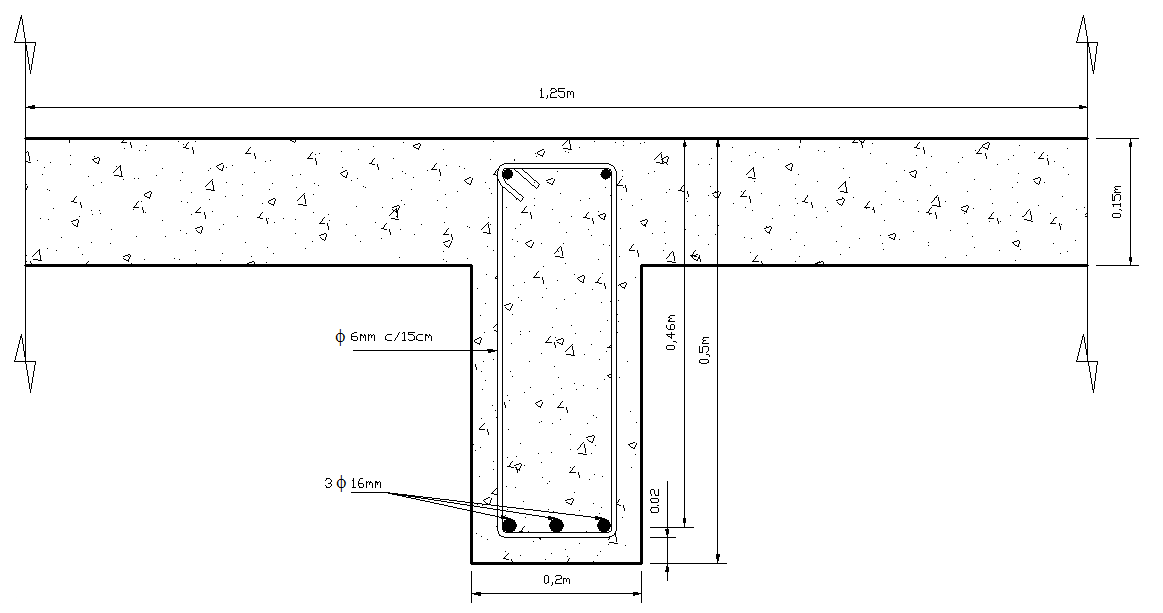
\includegraphics[scale = 0.6]{chapters/chapter_1/images/figura6.png}
     \caption{Sección Viga T}
\end{center}
\end{figure}

\newpage
\item \underline{Verificar el momemnto último de una viga}

\underline{Datos:}\\
\begin{align*}
& \text{Hormigón H20}\Rightarrow f'c = 20MPa\\
& \text{Acero ADN 42/50}\Rightarrow fy = 420MPa\\
& 4 \phi 16mm \quad\text{inferior} \Rightarrow 8.04 cm^2\\
& b_w = 20 cm\\
& d = 0.56 m\\
& h = 0.6m
\end{align*}

\begin{align*}
& a = \frac{As \cdot fy}{0.85 \cdot f'c \cdot b_w} = \frac{8.04 cm^2 \cdot 420MPa}{0.85 \cdot 20MPa \cdot 20 cm} = \framebox{9.93 cm}\\
& Ka = \frac{a}{d} = \frac{9.93 cm}{56 cm} = \framebox{0.177}\\
& Ka_{min}= \frac{1.4}{0.85 \cdot f'c} = \frac{1.4}{0.85 \cdot 20MPa} = \framebox{0.082}\\
& Ka_{max}= 0.375 \cdot \beta_1 = 0.375 \cdot 0.85 = \framebox{0.3187}\\
& Ka_{min} < Ka < Ka_{max}\\
& 0.082 < 0.177 < 0.3187 \Rightarrow \quad \text{Verifica} \quad \surd\\
& M_n = 0.85 \cdot f'c \cdot b_w \cdot Ka \cdot d^2 \cdot (1- \frac{Ka}{2})\\
& M_n = 0.85 \cdot 20000 \frac{KN}{m^2} \cdot 0.2m \cdot 0.177 \cdot (0.56 m)^2 \cdot (1- \frac{0.177}{2}) = \framebox{172 KN.m}\\
& M_u = \phi \cdot M_n = 0.9 \cdot 172 KN.m = \framebox{154 KN.m}
\end{align*}

\begin{figure}[H]
\begin{center}
     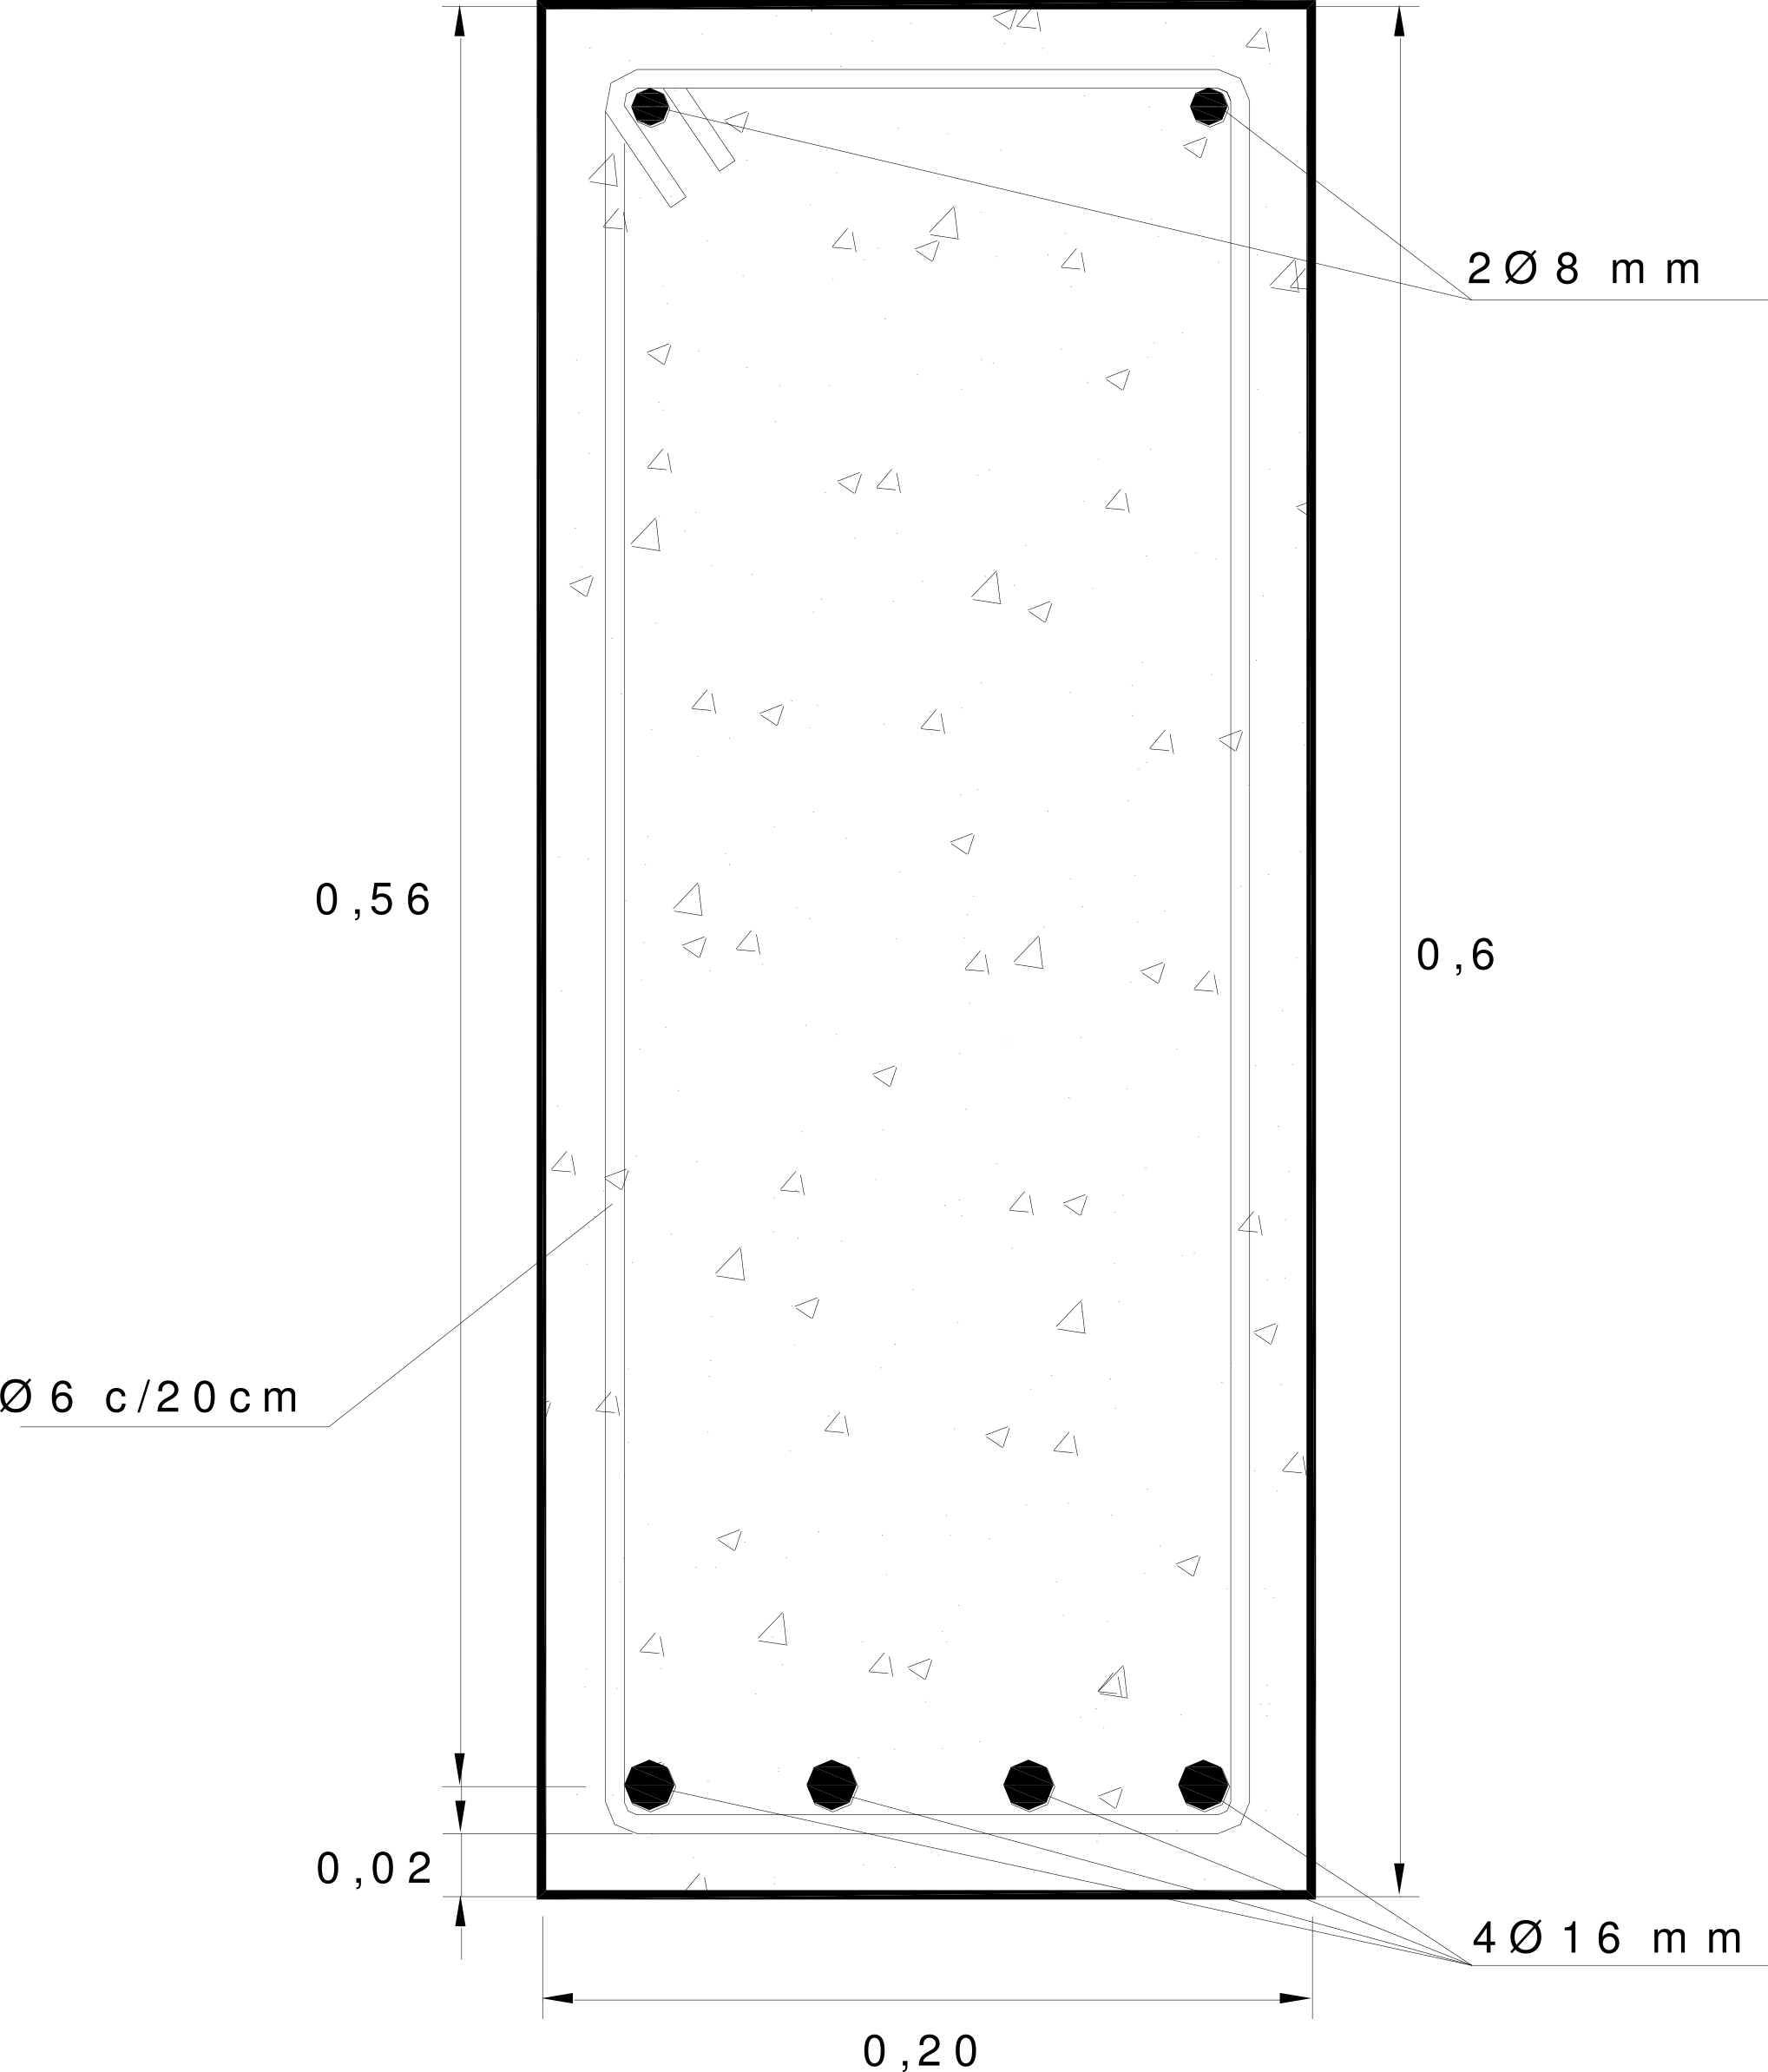
\includegraphics[scale = 0.9]{chapters/chapter_1/images/figura2.png}
     \caption{Sección de la viga}
\end{center}
\end{figure}

\end{enumerate}